\chapter{अकूटलेखी RNA और अनुलेखनोत्तर नियमन}\label{ch:b3:rna-regulation}

1990 में दो वनस्पति-जीवविज्ञानियों ने पिटूनिया को और गहरा बैंगनी बनाने
के लिए उन्हें वर्णक-एंज़ाइम के जीन की अतिरिक्त प्रतियाँ दीं। लगभग आधे
पारजीनी पौधे सफ़ेद निकले, या बैंगनी पर सफ़ेद खंडों वाले: जोड़े गए जीन
ने अपने साथ-साथ पौधे की अपनी प्रति भी बंद कर दी थी। आठ वर्ष बाद,
\emph{Caenorhabditis elegans} में RNA अंतःक्षेपित करते दो कृमि-आनुवंशिकीविदों
ने पाया कि किसी पेशी-जीन से मेल खाता द्विलड़ी RNA उस जीन को, अंतःक्षेपित
कृमि में और उसकी संतति में, अकेली किसी भी लड़ी की तुलना में कहीं अधिक
प्रबलता से मौन कर देता है। दोनों पहेलियों का एक ही उत्तर था: कोशिकाओं
के पास ऐसा तंत्र है जो छोटे RNA से मेल खाते अनुक्रम वाले RNA ढूँढ़कर
मौन कर देता है। वही तंत्र, और नियमन का वह व्यापक संसार जो किसी संदेशवाहक
RNA के अनुलेखित हो जाने के बाद उस पर बीतता है --- उसका विच्छेदन कैसे
होता है, उसे कहाँ भेजा जाता है, वह कितना जीता है, उसका अनुवादन होता है
या नहीं --- इस अध्याय का विषय है। वर्ष 1 के खंड ने जीन को ऐसी इकाई
माना था जो अपने प्रवर्तक पर चालू या बंद रहती है; यहाँ स्वयं अनुलेख
नियंत्रण का विषय बन जाता है।

\section{किसी कोशिका की RNA जनगणना}

\begin{definition}[अकूटलेखी RNA]\label{def:b3:rna-regulation:ncrna}
\index{अकूटलेखी RNA}\index{माइक्रो RNA}\index{siRNA}\index{piRNA}\index{दीर्घ अकूटलेखी RNA}\index{लघु केंद्रकीय RNA}
\emph{अकूटलेखी RNA} (ncRNA) वह अनुलेख है जो प्रोटीन के साँचे के रूप
में नहीं, स्वयं RNA के रूप में काम करता है। अनुवादन के राइबोसोमी तथा
अंतरण RNA और विच्छेदन-काय के \emph{लघु केंद्रकीय RNA} (snRNA) के आगे,
किसी सुकेंद्रकी कोशिका में ये होते हैं: \emph{माइक्रो RNA}
(miRNA), \numrange{21}{23} न्यूक्लियोटाइड के, जो कोशिका के अपने
अनुलेखों की हेयरपिनों से काटे जाते हैं और आंशिक रूप से पूरक संदेशवाहकों
के दमन का मार्गदर्शन करते हैं; \emph{लघु व्यवधानी RNA} (siRNA), उतने ही
लंबे, जो लंबे द्विलड़ी RNA से काटे जाते हैं और पूर्णतः मेल खाते
लक्ष्यों के विदलन का मार्गदर्शन करते हैं; \emph{Piwi-अन्योन्यकारी RNA}
(piRNA), \numrange{26}{31} न्यूक्लियोटाइड के, जो जनन-वंश में
ट्रांसपोज़ॉनों के विरुद्ध सक्रिय हैं; लघु केंद्रिकीय RNA, जो rRNA के
रूपांतरण का मार्गदर्शन करते हैं; और \emph{दीर्घ अकूटलेखी RNA} (lncRNA),
\qty{200}{nt} से लंबे ऐसे अनुलेख जिनमें कोई उल्लेखनीय खुला वाचन-ढाँचा
नहीं, जिनमें \cref{ch:b3:chromatin-epigenetics} का \emph{\omterm{def:b3:chromatin-epigenetics:x-inactivation}{Xist}} सबसे
अच्छी तरह समझा गया है। प्रोटीन-कूटलेखी बहिर्वेशन मानव जीनोम का लगभग
\qty{1.5}{\%} हैं; शेष का बड़ा अंश किसी न किसी समय किसी न किसी कोशिका
में अनुलेखित होता है, पर उस अनुलेखन का कितना भाग प्रकार्यात्मक है, यह
खुला प्रश्न है।
\end{definition}

\begin{remark}[बहुतायत प्रकार्य नहीं है]\label{rem:b3:rna-regulation:function}
कोई अनुलेख इसलिए भी पकड़ा जा सकता है कि पॉलीमरेज़ रिसती है, इसलिए नहीं
कि RNA कुछ करता है; अधिकांश lncRNA प्रति कोशिका एक प्रति से भी कम
मात्रा में हैं, कम संरक्षित हैं, और हटा देने पर अनावश्यक सिद्ध होते
हैं। प्रकार्य की कसौटी आनुवंशिक है: जब RNA हटे, न कि केवल उसका DNA, तब
कोई लक्षण-प्ररूप दिखे। \emph{\omterm{def:b3:chromatin-epigenetics:x-inactivation}{Xist}}, miRNA और \omterm{def:b3:rna-regulation:ncrna}{piRNA} इसे निर्णायक रूप से
पार करते हैं; अब तक टिप्पणीकृत हज़ारों lncRNA में से कुछ सौ ने ही ऐसा
किया है।
\end{remark}

\section{RNA व्यवधान और माइक्रो RNA}

\begin{definition}[RNA व्यवधान]\label{def:b3:rna-regulation:rnai}
\index{RNA व्यवधान}\index{डाइसर}\index{आर्गोनॉट}\index{RISC}
\emph{RNA व्यवधान} (RNAi) द्विलड़ी RNA से बने किसी छोटे RNA द्वारा किसी
जीन का अनुक्रम-विशिष्ट मौनीकरण है। एंज़ाइम \emph{डाइसर}, एक RNase III,
लंबे द्विलड़ी RNA को \numrange{21}{23}-न्यूक्लियोटाइड के ऐसे युग्मकों
में काटती है जिनके 3$'$ सिरों पर दो-न्यूक्लियोटाइड के अधिलंब हैं; हर
युग्मक की एक लड़ी, मार्गदर्शक, किसी \emph{आर्गोनॉट} प्रोटीन में भरी
जाती है और \emph{RNA-प्रेरित मौनीकरण संकुल} (RISC) बनता है।
मार्गदर्शक किसी पूरक लक्ष्य RNA से युग्मित होता है, और आर्गोनॉट का
एंडोन्यूक्लिएज़ प्रांत लक्ष्य को मार्गदर्शक के न्यूक्लियोटाइड 10 तथा
11 के सामने काट देता है; कटा RNA फिर अपघटित होता है और RISC मुक्त
होकर कोई दूसरा ढूँढ़ता है। पौधों, कृमियों और कवकों में एक RNA-निर्भर
RNA पॉलीमरेज़ लक्ष्य की नकल करके नया द्विलड़ी RNA बनाती है, जिससे संकेत
प्रवर्धित होकर फैलता है; स्तनधारियों में यह चरण नहीं है।
\end{definition}

\begin{proof}[प्रमाण-सामग्री]
नेपोली, लेमीयू और योर्गेनसन (1990) ने फूल का रंग गाढ़ा करने के लिए
पिटूनिया में चैल्कोन सिंथेज़ का एक अतिरिक्त जीन डाला; \qty{42}{\%}
रूपांतरित पौधे सफ़ेद या चितकबरे निकले, जिनमें पारजीन और अंतर्जात जीन
दोनों मौन थे --- ``सह-दमन''। गुओ और केम्फ़्यूस (1995) ने पाया कि किसी
\emph{C.~elegans} जीन के विरुद्ध प्रतिसंवेदी RNA ने उसे मौन किया, पर
संवेदी नियंत्रण ने भी वही किया। फ़ायर, मेलो और सहयोगियों (1998) ने
विरोधाभास सुलझाया: उनकी एकल-लड़ी तैयारियाँ द्विलड़ियों से दूषित थीं, और
\emph{unc-22} का शुद्ध द्विलड़ी RNA किसी कृमि में अंतःक्षेपित करने पर
प्रति कोशिका कुछ ही अणुओं की सांद्रता पर \emph{unc-22} का फड़कने वाला
लक्षण-प्ररूप दे देता था, जबकि शुद्ध संवेदी या प्रतिसंवेदी RNA से लगभग
कुछ नहीं होता था; मौनीकरण अंतःक्षेपण-स्थल से दूर के ऊतकों में और संतति
में भी पहुँचा। हैमिल्टन और बॉलकोम (1999) ने मौन किए गए पौधों में
\qty{25}{nt} के RNA पकड़े, और ज़ामोर तथा सहयोगियों (2000) ने किसी मक्खी
के निष्कर्ष में दिखाया कि द्विलड़ी RNA उन्हीं में कटता है और लक्ष्य
\qty{21}{nt} के अंतरालों पर विदलित होता है।
\end{proof}

\begin{omfigure}
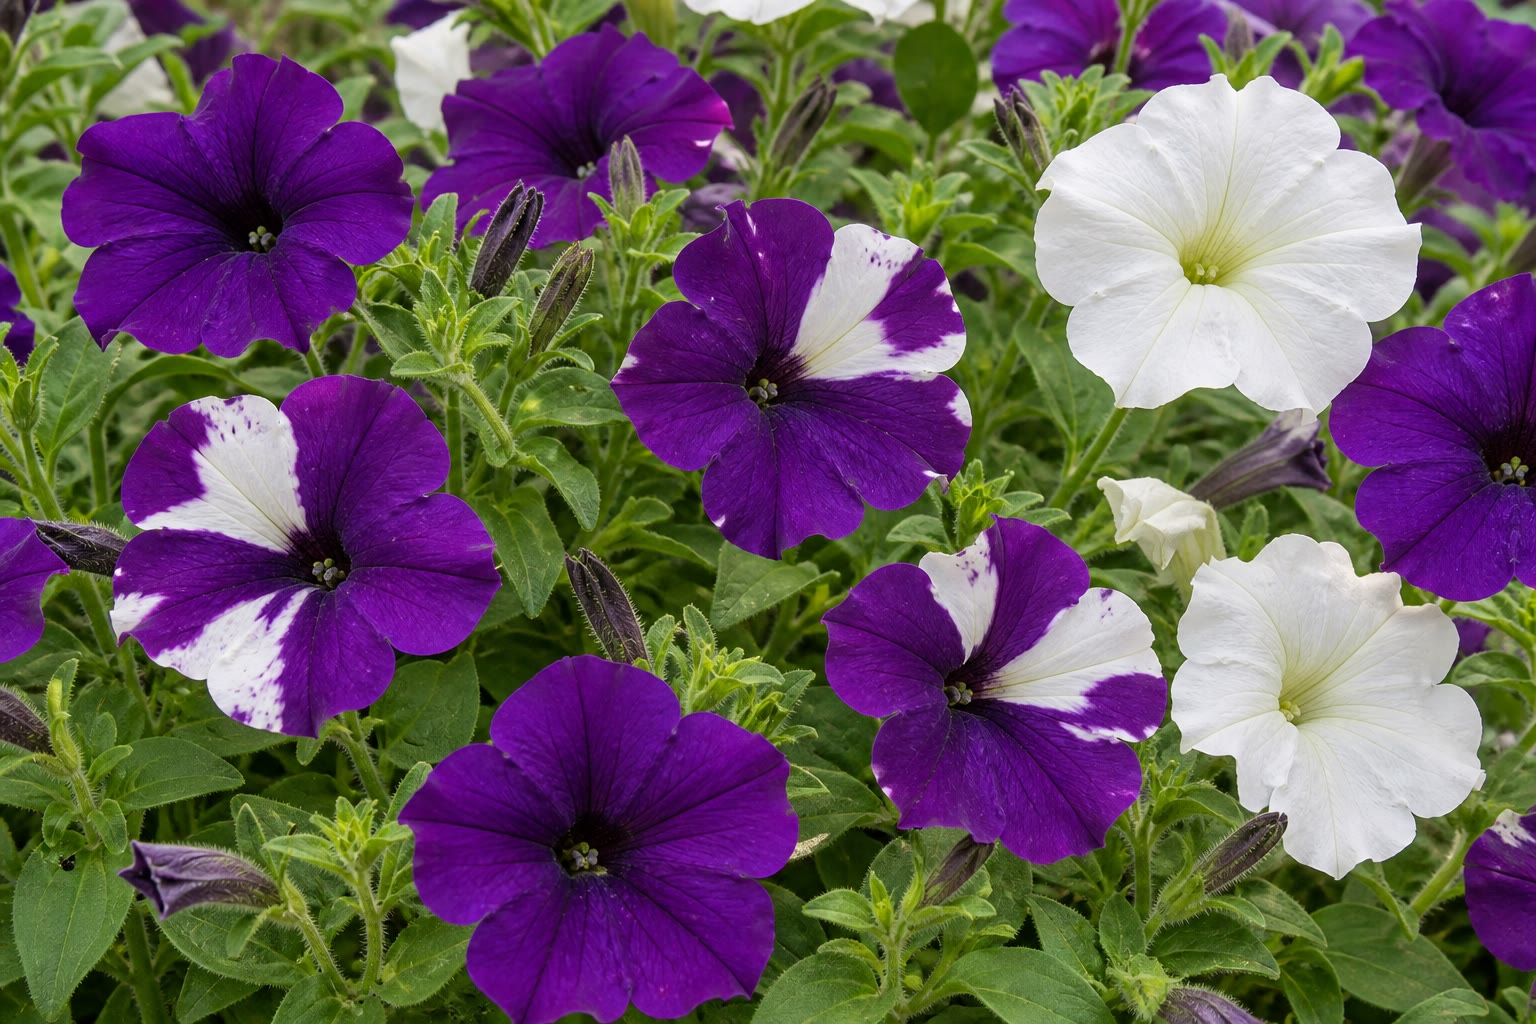
\includegraphics[width=0.46\linewidth]{images/book5/ai/b5-02-petunia-cosuppression.jpg}\hspace{0.04\linewidth}
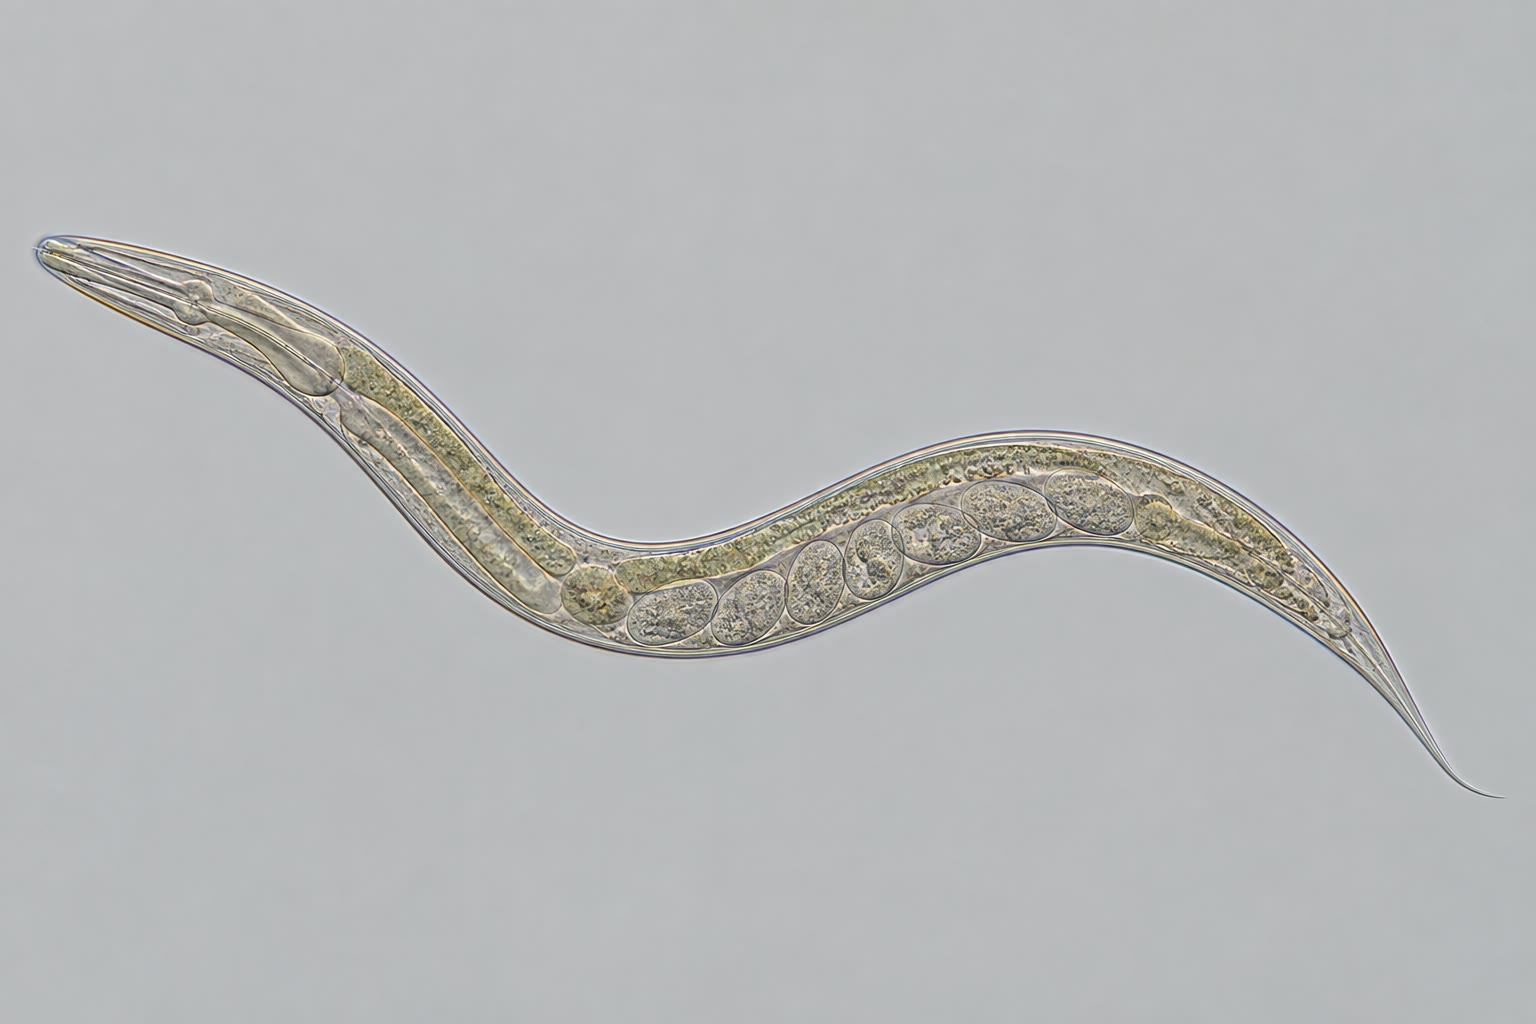
\includegraphics[width=0.46\linewidth]{images/book5/ai/b5-02-c-elegans.jpg}

{\small बाएँ: अतिरिक्त वर्णक-जीन ढोते पिटूनिया, जिन पर सह-दमन के सफ़ेद
खंड हैं। दाएँ: सूत्रकृमि \emph{Caenorhabditis
elegans}, लगभग एक मिलीमीटर लंबा और पारदर्शी, जिसमें अंतःक्षेपित
द्विलड़ी RNA ने पूरे प्राणी में और उसकी संतति में मेल खाता जीन मौन कर
दिया।}
\end{omfigure}

\begin{definition}[माइक्रो RNA]\label{def:b3:rna-regulation:mirna}
\index{माइक्रो RNA!जीवसंश्लेषण}\index{ड्रोशा}\index{बीज अनुक्रम}
कोई \emph{\omterm{def:b3:rna-regulation:ncrna}{माइक्रो RNA}} जीनोम में कूटबद्ध होता है --- अपने ही जीन में या
किसी प्रोटीन-कूटलेखी जीन के अंतर्वेशन में --- और RNA पॉलीमरेज़ II
द्वारा एक लंबे प्राथमिक अनुलेख (pri-miRNA) के रूप में अनुलेखित होता है,
जिसमें लगभग \qty{70}{nt} की एक हेयरपिन होती है। केंद्रक में RNase III
\emph{ड्रोशा} अपने साथी DGCR8 के साथ हेयरपिन को काटकर निकालती है
(pre-miRNA); एक्सपोर्टिन-5 उसे कोशिकाद्रव्य तक ले जाता है, जहाँ \omterm{def:b3:rna-regulation:rnai}{डाइसर}
फंदा हटा देती है और \qty{22}{nt} का युग्मक बचता है। एक लड़ी \omterm{def:b3:rna-regulation:rnai}{आर्गोनॉट}
में भरी जाती है। परिपक्व miRNA अपने लक्ष्य मुख्यतः अपने \emph{बीज} से
पहचानता है, यानी न्यूक्लियोटाइड 2 से 8 से, जो प्रायः किसी संदेशवाहक के
3$'$ अननुवादित क्षेत्र के स्थलों से युग्मित होते हैं; miRNA का शेष भाग
अपूर्ण रूप से युग्मित होता है, इसलिए लक्ष्य विदलित नहीं होता बल्कि दमित
होता है: \omterm{def:b3:rna-regulation:rnai}{RISC} ऐसे प्रोटीन बुलाता है जो पॉली(A) पुच्छ छोटी करते हैं,
टोपी हटाते हैं और अनुवादन रोकते हैं, और संदेशवाहक तेज़ी से अपघटित होता
है। चूँकि कोई बीज केवल सात न्यूक्लियोटाइड का है, एक ही miRNA के सैकड़ों
लक्ष्य होते हैं, और आधे से अधिक मानव प्रोटीन-कूटलेखी जीनों पर कुछ सौ
विश्वसनीय रूप से पहचाने गए मानव miRNA में से कम-से-कम एक के लिए
संरक्षित स्थल हैं।
\end{definition}

\begin{proof}[प्रमाण-सामग्री]
\emph{lin-4}, वह जीन जो कृमि को पहली डिंभ अवस्था से दूसरी तक बढ़ने के
लिए चाहिए, ली, फ़ाइनबॉम और ऐम्ब्रोस (1993) को ऐसा मिला जो किसी प्रोटीन
का नहीं बल्कि \qty{22}{nt} के एक RNA का कूटलेखन करता है, जो
\emph{lin-14} के संदेशवाहक के 3$'$ अननुवादित क्षेत्र के सात स्थलों का
पूरक है --- वही जीन जिसे वह दमित करता जाना जाता था। जैसे ही डिंभ दूसरी
अवस्था में प्रवेश करता है, LIN-14 प्रोटीन लुप्त हो जाता है जबकि उसका
mRNA बना रहता है: दमन अनुलेखनोत्तर है। राइनहार्ट और सहयोगियों (2000) ने
ऐसा ही एक दूसरा RNA, \emph{let-7}, पाया, जो बाद की डिंभ-संक्रांतियों
को नियंत्रित करता है; पास्क्वीनेली (2000) ने \emph{let-7} को मक्खियों
और मनुष्यों में उसी अनुक्रम के साथ पाया, जिसने किसी कृमि की
विचित्रता को एक सामान्य क्रियाविधि बना दिया।
\end{proof}

\begin{omfigure}
\begin{tikzpicture}[every node/.style={font=\scriptsize}, >=stealth]
  % nucleus box
  \draw[rounded corners=8pt, thick, gray!60, fill=gray!6] (-0.4,-1.1) rectangle (5.2,2.7);
  \node[gray, anchor=south west] at (-0.3,-1.05) {केंद्रक};
  % gene and pri-miRNA
  \draw[very thick, omDef] (0,2.0) -- (2.4,2.0); \node[above] at (1.2,2.05) {miRNA जीन, Pol II};
  \draw[->, thick] (1.2,1.85) -- (1.2,1.35);
  % hairpin
  \draw[thick, omThm!70!black] (0.2,1.0) -- (0.9,1.0) .. controls (1.0,1.0) and (1.05,0.9) .. (1.1,0.5) .. controls (1.15,0.1) and (1.25,0.1) .. (1.3,0.5) .. controls (1.35,0.9) and (1.4,1.0) .. (1.5,1.0) -- (2.2,1.0);
  \draw[thick, omThm!70!black] (1.1,0.5) -- (1.3,0.5);
  \node[below] at (1.2,0.0) {pri-miRNA हेयरपिन};
  % Drosha
  \draw[thick, fill=omExo!35] (2.9,0.7) ellipse (0.55 and 0.28); \node at (2.9,0.7) {ड्रोशा};
  \draw[->, thick] (2.3,0.85) -- (2.4,0.75);
  \draw[->, thick] (3.5,0.7) -- (4.2,0.7) node[midway, above] {कटाई};
  % pre-miRNA
  \draw[thick, omThm!70!black] (4.3,0.9) .. controls (4.5,0.9) and (4.55,0.4) .. (4.6,0.1) .. controls (4.65,-0.2) and (4.75,-0.2) .. (4.8,0.1) .. controls (4.85,0.4) and (4.9,0.9) .. (5.1,0.9);
  \node[below, align=center] at (4.7,-0.25) {pre-miRNA\\\qty{70}{nt}};
  % export
  \draw[->, thick] (5.35,0.4) -- (6.3,0.4) node[midway, above, xshift=0.2cm] {एक्सपोर्टिन-5};
  % cytoplasm
  \node[gray, anchor=north west] at (5.5,2.65) {कोशिकाद्रव्य};
  \draw[thick, fill=omExo!35] (6.9,0.4) ellipse (0.5 and 0.28); \node at (6.9,0.4) {डाइसर};
  \draw[->, thick] (7.45,0.4) -- (8.1,0.4);
  \draw[thick, omThm!70!black] (8.2,0.55) -- (9.6,0.55); \draw[thick, omThm!70!black] (8.35,0.25) -- (9.75,0.25);
  \node[below, align=center] at (8.95,0.15) {\qty{22}{nt} युग्मक};
  \draw[->, thick] (8.95,-0.4) -- (8.95,-0.9) node[midway, right] {एक लड़ी भरी जाती है};
  % RISC on mRNA
  \draw[thick, fill=omProp!35] (8.95,-1.45) ellipse (0.85 and 0.35); \node at (8.95,-1.45) {आर्गोनॉट};
  \draw[thick, omThm!70!black] (8.3,-1.85) -- (9.6,-1.85);
  \draw[very thick, omDef] (5.6,-2.15) -- (11.4,-2.15);
  \node[below] at (6.4,-2.2) {mRNA: कूटलेखी क्षेत्र}; \node[below] at (10.3,-2.2) {3$'$ UTR, लक्ष्य स्थल};
  \draw[omDef, thick] (11.4,-2.15) -- (11.8,-2.15) node[right] {AAAA};
  \draw[->, thick, omThm] (9.9,-1.5) -- (10.9,-1.5) node[right, align=left] {अपऐडीनिलन,\\क्षय, कम\\अनुवादन};
  \node[below, align=center] at (8.95,-2.7) {बीज (nt 2--8) स्थल से\\युग्मित होता है};
\end{tikzpicture}

{\small किसी \omterm{def:b3:rna-regulation:ncrna}{माइक्रो RNA} का जीवसंश्लेषण। हेयरपिन को केंद्रक में \omterm{def:b3:rna-regulation:mirna}{ड्रोशा}
प्राथमिक अनुलेख से काटकर निकालती है, वह निर्यात होती है, \omterm{def:b3:rna-regulation:rnai}{डाइसर} उसे
छाँटकर \qty{22}{nt} का युग्मक बनाती है, और एक लड़ी \omterm{def:b3:rna-regulation:rnai}{आर्गोनॉट} में भरी
जाती है। बीज किसी संदेशवाहक के 3$'$ अननुवादित क्षेत्र के स्थल से
युग्मित होता है और संदेशवाहक अपऐडीनिलित, अपघटित और कम अनुवादित होता है।}
\end{omfigure}

\begin{theorem}[कोई माइक्रो RNA किसी संदेशवाहक के स्तर और गति के साथ क्या करता है]\label{thm:b3:rna-regulation:mirna-kinetics}
\index{mRNA अर्ध-आयु}\index{अनुक्रिया-काल}
कोई संदेशवाहक अचर दर $k$ से संश्लेषित होता है और प्रथम-कोटि दर
$\gamma$ से अपघटित; स्तर $R$ पर उपस्थित कोई \omterm{def:b3:rna-regulation:ncrna}{माइक्रो RNA} एक क्षय-पद
$\gamma' R\, m$ जोड़ देता है। तब mRNA स्तर $m(t)$ इसका पालन करता है
\[
\frac{\mathrm{d}m}{\mathrm{d}t} = k - (\gamma + \gamma' R)\, m,
\qquad
m^{*} = \frac{k}{\gamma + \gamma' R},
\qquad
m(t) = m^{*} + (m_{0} - m^{*})\,e^{-(\gamma + \gamma' R)t}.
\]
\omterm{def:b3:rna-regulation:ncrna}{माइक्रो RNA} स्थायी अवस्था को $1 + \gamma' R/
\gamma$ गुणक से घटाता है और $m$ में हर बदलाव का काल-नियतांक उसी गुणक
से $1/\gamma$ से घटाकर $1/(\gamma + \gamma' R)$ कर देता है। इसलिए
माइक्रो-RNA-नियंत्रित कोई जीन अधिक शांत भी है और अधिक तेज़ भी: अपने
प्रवर्तक के बदलने के बाद वह नई स्थायी अवस्था तक जल्दी पहुँचता है, और
उसके अनुलेखन के उतार-चढ़ाव दब जाते हैं।
\end{theorem}
\begin{proof}
समीकरण अचर गुणांकों वाला रैखिक समीकरण है; उसका स्थिर बिंदु वहाँ
$m^{*}$ है जहाँ दायाँ पक्ष लुप्त होता है, और $u = m - m^{*}$ लिखने पर
$\mathrm{d}u/\mathrm{d}t = -(\gamma + \gamma' R)\,u$ मिलता है, जिससे
चरघातांकी रूप आता है। पहुँच का अर्ध-काल $\ln 2/(\gamma + \gamma'
R)$ है, और $\gamma = \ln 2 / t_{1/2}$, जहाँ $t_{1/2}$ संदेशवाहक का
प्राकृतिक अर्ध-आयु काल है।
\end{proof}

\begin{example}[चार गुना दमन]\label{ex:b3:rna-regulation:fourfold}
\qty{30}{min} के प्राकृतिक अर्ध-आयु काल वाला कोई संदेशवाहक ($\gamma =
\qty{0.023}{min^{-1}}$), जो $k = 2$ अणु प्रति मिनट की दर से अनुलेखित
होता है, $m^{*} = 2/0.023 \approx 87$ प्रतियाँ प्रति कोशिका पर बैठता है
और अपने प्रवर्तक के बदलने के बाद किसी नए स्तर तक आधा रास्ता तय करने में
\qty{30}{min} लेता है। जो \omterm{def:b3:rna-regulation:ncrna}{माइक्रो RNA} उसकी क्षय-दर तिगुनी कर देता है
($\gamma' R = 3\gamma$) वह उसे $22$ प्रतियों तक ले आता है और अर्ध-काल
घटाकर \qty{7.5}{min} कर देता है। यही संख्याएँ उलटी पढ़ें तो दिखाती हैं
कि miRNA निष्क्रियणों के लक्षण-प्ररूप प्रायः हल्के क्यों होते हैं: किसी
ऐसे संदेशवाहक में चार गुना बदलाव जो आगे स्वयं प्रतिरोधित है, जीव को
लगभग सामान्य छोड़ सकता है, और प्रभाव तनाव में या समय-नियोजन में दिखता
है।
\end{example}

\begin{omfigure}
\begin{tikzpicture}
\begin{axis}[
  width=0.7\linewidth, height=5.6cm,
  axis x line=bottom, axis y line=left,
  xmin=0, xmax=120, ymin=0, ymax=100,
  xlabel={प्रवर्तक के चालू होने के बाद का समय (min)}, ylabel={mRNA प्रति कोशिका},
  xlabel style={font=\small, at={(axis description cs:0.5,-0.12)}, anchor=north},
  ylabel style={font=\small},
  tick label style={font=\small}, xtick={0,30,60,90,120}, ytick={0,22,50,87},
  clip=false,
]
\addplot[very thick, omDef, domain=0:120, samples=80] {87*(1-exp(-0.0231*x))};
\addplot[very thick, omThm, domain=0:120, samples=80] {21.7*(1-exp(-0.0924*x))};
\addplot[dashed, gray, domain=0:120, samples=2] {87};
\addplot[dashed, gray, domain=0:120, samples=2] {21.7};
\node[font=\scriptsize, omDef, anchor=south west] at (axis cs:5,90) {माइक्रो RNA नहीं: $m^{*} = 87$, अर्ध-काल \qty{30}{min}};
\node[font=\scriptsize, omThm, anchor=south west] at (axis cs:40,24) {माइक्रो RNA के साथ, $\gamma' R = 3\gamma$: $m^{*} = 22$, अर्ध-काल \qty{7.5}{min}};
\end{axis}
\end{tikzpicture}

{\small \cref{ex:b3:rna-regulation:fourfold} की संख्याओं के साथ, अपने
प्रवर्तक के चालू होने के बाद किसी संदेशवाहक का उठान। \omterm{def:b3:rna-regulation:ncrna}{माइक्रो RNA}
पठार को चार गुना नीचे लाता है और उस तक चार गुना जल्दी पहुँचता है।}
\end{omfigure}

\begin{method}[RNAi से किसी जीन को दबाना]\label{met:b3:rna-regulation:knockdown}
\index{अवदमन}\index{shRNA}
किसी जीन को उसके DNA को छुए बिना मौन करने के लिए: (1) उसके संदेशवाहक
के लिए अनन्य कोई \qty{21}{nt} अनुक्रम चुनिए, दूसरे जीनों से बीज-मेल से
बचते हुए; (2) उसे संश्लेषित \omterm{def:b3:rna-regulation:ncrna}{siRNA} युग्मक के रूप में (क्षणिक, कुछ दिन)
या किसी संवाहक से अभिव्यक्त लघु हेयरपिन RNA (shRNA) के रूप में
पहुँचाइए, जिसे \omterm{def:b3:rna-regulation:rnai}{डाइसर} लगातार संसाधित करती है; कृमियों में प्राणियों को
द्विलड़ी RNA अभिव्यक्त करते जीवाणु खिलाइए; (3) संदेशवाहक को मात्रात्मक
PCR से और प्रोटीन को प्रतिरक्षा-ब्लॉट से मापिए, और किसी निष्क्रियण की
पूर्ण अनुपस्थिति के बजाय \qtyrange{70}{95}{\%} ह्रास की अपेक्षा
रखिए; (4) लक्ष्येतर प्रभावों के लिए दूसरे, अनतिव्यापी \omterm{def:b3:rna-regulation:ncrna}{siRNA} से और जीन
के किसी RNAi-प्रतिरोधी रूप से पुनरुद्धार करके नियंत्रण रखिए। अवदमन
प्रकार्य का आंशिक, उत्क्रमणीय ह्रास है; इस सिद्धांत पर अब तक स्वीकृत
जीन-चिकित्साएँ यकृत के संदेशवाहकों (ट्रांसथाइरेटिन, PCSK9) के विरुद्ध
\omterm{def:b3:rna-regulation:ncrna}{siRNA} को ऐसी शर्करा से जोड़कर पहुँचाती हैं जिसे यकृत-कोशिका ग्रहण कर
लेती है।
\end{method}

\section{जीनोम की रक्षा करने वाले छोटे RNA}

\begin{definition}[piRNA और ट्रांसपोज़ॉन मौनीकरण]\label{def:b3:rna-regulation:pirna}
\index{piRNA!पिंग-पॉन्ग}\index{ट्रांसपोज़ॉन मौनीकरण}\index{संकर दुर्जननता}
\emph{\omterm{def:b3:rna-regulation:ncrna}{piRNA}} \numrange{26}{31}-न्यूक्लियोटाइड के ऐसे RNA हैं जो \omterm{def:b3:rna-regulation:rnai}{डाइसर}
के बिना, जीनोमी \emph{\omterm{def:b3:rna-regulation:ncrna}{piRNA} गुच्छों} --- दोषपूर्ण ट्रांसपोज़ॉन
प्रतियों के कब्रिस्तानों --- के लंबे एकलड़ी अनुलेखों से बनते हैं और
जनन-वंश में \omterm{def:b3:rna-regulation:rnai}{आर्गोनॉट} प्रोटीनों के PIWI उपकुल में भरे जाते हैं। किसी
ट्रांसपोज़ॉन का प्रतिसंवेदी \omterm{def:b3:rna-regulation:ncrna}{piRNA} उस ट्रांसपोज़ॉन के अनुलेखों के विदलन
का मार्गदर्शन करता है; कटा खंड नया संवेदी \omterm{def:b3:rna-regulation:ncrna}{piRNA} बन जाता है, जो बदले में
गुच्छा-अनुलेखों को काटकर और प्रतिसंवेदी \omterm{def:b3:rna-regulation:ncrna}{piRNA} बनाता है --- यही
\emph{पिंग-पॉन्ग} चक्र है, एक ऐसा प्रवर्धन जो उसी ट्रांसपोज़ॉन को
निशाना बनाता है जो इस समय सक्रिय हो। केंद्रकीय PIWI प्रोटीन
ट्रांसपोज़ॉन की जीनोमी प्रतियों पर H3K9 मेथिलीकरण और \omterm{def:b3:chromatin-epigenetics:methylation}{DNA मेथिलीकरण} भी
निर्देशित करते हैं, जिससे RNA \cref{ch:b3:chromatin-epigenetics} के
\omterm{def:b3:chromatin-epigenetics:nucleosome}{क्रोमैटिन} चिह्नों से जुड़ जाता है। कोई माता अपने \omterm{def:b3:rna-regulation:ncrna}{piRNA} अंडाणु में जमा
करती है; जिस मादा के वंशक्रम ने कभी कोई ट्रांसपोज़ॉन नहीं देखा उसके पास
उसके विरुद्ध कोई \omterm{def:b3:rna-regulation:ncrna}{piRNA} नहीं होता, और उसे ढोने वाले किसी नर से उसकी
संतति बंध्य होती है --- \emph{संकर दुर्जननता}, जो सबसे पहले प्रयोगशाला
और वन्य प्रजातियों के बीच \emph{Drosophila} संकरणों में देखी गई।
\end{definition}

\begin{proposition}[RNA-निर्देशित क्रोमैटिन मौनीकरण]\label{prop:b3:rna-regulation:rddm}
\index{RNA-निर्देशित DNA मेथिलीकरण}
पौधों में एक समर्पित पथ --- RNA पॉलीमरेज़ IV किसी स्थल का अनुलेखन करती
है, कोई RNA-निर्भर RNA पॉलीमरेज़ उसे द्विलड़ी बनाती है, कोई \omterm{def:b3:rna-regulation:rnai}{डाइसर}
\qty{24}{nt} के \omterm{def:b3:rna-regulation:ncrna}{siRNA} काटती है, \omterm{def:b3:rna-regulation:rnai}{आर्गोनॉट}~4 उन्हें उसी स्थल पर
पॉलीमरेज़ V के नवजात अनुलेखों तक वापस ले जाता है और मेथिलट्रांसफ़रेज़
DRM2 को बुलाता है --- ट्रांसपोज़ॉनों और पुनरावर्ती अनुक्रमों के DNA का
मेथिलीकरण करता है; यही परा-उत्परिवर्तन की क्रियाविधि है। विखंडन खमीर
में गुणसूत्रबिंदु की पुनरावृत्तियों से बने \omterm{def:b3:rna-regulation:ncrna}{siRNA} H3K9
मेथिलट्रांसफ़रेज़ को बुलाते हैं और वह \omterm{def:b3:chromatin-epigenetics:nucleosome}{विषमक्रोमैटिन} बनाते हैं जो
गुणसूत्रबिंदु को चाहिए। दोनों स्थितियों में कोई RNA पूरकता से जीनोम में
अपनी जगह ढूँढ़ता है और वहाँ कोई \omterm{def:b3:chromatin-epigenetics:nucleosome}{क्रोमैटिन} चिह्न लिखा जाता है:
अनुक्रम-विशिष्ट, स्वयं-सुदृढ़, और विभाजनों के पार वंशागत।
\end{proposition}

\section{किसी संदेशवाहक का जीवन}

\begin{definition}[नियमित विच्छेदन]\label{def:b3:rna-regulation:splicing}
\index{वैकल्पिक विच्छेदन!नियमन}\index{SR प्रोटीन}\index{hnRNP}\index{बहिर्वेशन लोप}
वैकल्पिक विच्छेदन एक ही जीन से भिन्न संदेशवाहक बनाता है ---
\emph{बहिर्वेशन लोप} से, परस्पर अपवर्जी बहिर्वेशनों के बीच चुनाव से,
किसी अंतर्वेशन को रोक रखने से, या वैकल्पिक 5$'$ अथवा 3$'$ विच्छेदन
स्थलों के उपयोग से। इसका नियमन वे RNA-बंधक प्रोटीन करते हैं जो किसी
विच्छेदन स्थल के पास बहिर्वेशनों और अंतर्वेशनों के अनुक्रम-अवयवों से
बँधते हैं: बहिर्वेशनी संवर्धकों से बँधे \emph{SR प्रोटीन}
विच्छेदन-काय को बुलाते हैं और बहिर्वेशन के समावेश को बढ़ावा देते हैं,
मौनकों से बँधे \emph{hnRNP} प्रोटीन उसे रोकते हैं, और किसी दी हुई
कोशिका में परिणाम दोनों प्रकारों की सापेक्ष मात्रा से तय होता है। मानव
बहु-बहिर्वेशनी जीनों में से \qty{90}{\%} से अधिक का वैकल्पिक विच्छेदन
होता है; \emph{Drosophila} का \emph{Dscam} जीन, जिसमें परस्पर अपवर्जी
बहिर्वेशनों के चार खंड हैं (12, 48, 33 और 2 विकल्प), \num{38016} भिन्न
प्रोटीन बना सकता है, और हर तंत्रिका-कोशिका एक भिन्न समुच्चय अभिव्यक्त
करती है जिससे उसकी शाखाएँ एक-दूसरे को पहचानकर बच सकें।
\end{definition}

\begin{proof}[प्रमाण-सामग्री]
किसी फल-मक्खी का लिंग एक विच्छेदन-प्रपात तय करता है। मादाओं में
\emph{Sex-lethal} (\emph{Sxl}) जीन एक प्रकार्यशील प्रोटीन बनाता है; SXL
एक RNA-बंधक प्रोटीन है जो अपने ही अनुलेख में एक विच्छेदन स्थल रोकता है
(जिससे विराम-कूटक वाला बहिर्वेशन छूट जाता है और प्रोटीन बनता रहता है)
और \emph{transformer} के अनुलेख में भी, जिससे मादा विच्छेदन बाध्य होता
है; फिर TRA, TRA-2 के साथ, \emph{doublesex} अनुलेख के किसी बहिर्वेशनी
संवर्धक से बँधता है और DSX अनुलेखन-कारक का मादा रूप निर्देशित करता है।
नरों में, जहाँ SXL नहीं होता, इनमें से हर अनुलेख चूक-विच्छेदन लेता है,
\emph{transformer} में एक विराम-कूटक आ जाता है, और DSX नर रूप में
निकलता है। मक्खी का हर लैंगिक द्विरूपी लक्षण इसी से निकलता है कि कौन-सा
DSX बना; जिस मादा में \emph{tra} उत्परिवर्तित है वह नर के रूप में
विकसित होती है।
\end{proof}

\begin{definition}[mRNA स्थायित्व और स्थानिकीकरण]\label{def:b3:rna-regulation:stability}
\index{AU-समृद्ध अवयव}\index{mRNA स्थानिकीकरण}\index{लौह-अनुक्रियक अवयव}
किसी संदेशवाहक का \emph{अर्ध-आयु काल} मिनटों से दिनों तक होता है और
उसके 3$'$ अननुवादित क्षेत्र के अवयव उसे तय करते हैं। साइटोकाइनों,
वृद्धि कारकों और आद्य-कर्कट जीनों के संदेशवाहकों में
\emph{AU-समृद्ध अवयवों} (AUUUA पुनरावृत्तियों) से ऐसे प्रोटीन बँधते हैं
जो अपऐडीनिलेज़ बुलाते हैं और \qtyrange{10}{30}{min} का अर्ध-आयु काल
देते हैं, ताकि अनुलेखन का एक स्फुरण प्रोटीन का एक स्फुरण दे और उससे
अधिक कुछ नहीं; उन्हें हटाने वाले उत्परिवर्तन अति-अभिव्यक्ति और, कुछ
आद्य-कर्कट जीनों के लिए, कर्कट पैदा करते हैं। \emph{स्थानिकीकरण अवयव},
प्रायः संरचित, ऐसे संयोजकों से बँधते हैं जो संदेशवाहक को किसी मोटर से
जोड़ देते हैं: \emph{bicoid} और \emph{oskar} संदेशवाहक सूक्ष्मनलिकाओं
पर डाइनीन और काइनेसिन से मक्खी के अंडे के दोनों ध्रुवों तक ले जाए जाते
हैं, $\beta$-ऐक्टिन संदेशवाहक किसी तंतुकोरक के अग्रणी किनारे तक, और
सूत्रयुग्मी प्रोटीनों के संदेशवाहक द्रुमिकाओं में, जहाँ माँग पर उनका
अनुवादन होता है। \emph{लौह-अनुक्रियक अवयव} (IRE), एक दंड--फंदा जिससे
लोहा दुर्लभ होने पर लौह-नियामक प्रोटीन IRP1 और IRP2 बँधते हैं, दो
स्थानों से दो उलटे काम करता है: फ़ेरिटिन संदेशवाहक के 5$'$ अननुवादित
क्षेत्र में बँधा IRP राइबोसोम को रोकता है; ट्रांसफ़ेरिन ग्राही के
संदेशवाहक के 3$'$ अननुवादित क्षेत्र में बँधा IRP अनुलेख को किसी
न्यूक्लिएज़ से बचाता है।
\end{definition}

\begin{example}[लोहा, एक ही हेयरपिन से पढ़ा गया]\label{ex:b3:rna-regulation:iron}
लोहा कम हो तो IRP दोनों संदेशवाहकों से बँधता है: भंडारण-प्रोटीन
फ़ेरिटिन का अनुवादन नहीं होता, और लोहा आयात करने वाला ट्रांसफ़ेरिन
ग्राही स्थिर तथा प्रचुर रहता है --- कोशिका कम भंडारण करती है और अधिक
आयात। लोहा अधिक हो तो वह IRP1 को ऐकोनिटेज़ में बदल देता है (वह एक
लौह--गंधक गुच्छ ले लेता है और अपनी RNA-आसक्ति खो देता है) और IRP2 का
अपघटन चालू कर देता है: फ़ेरिटिन का अनुवादन होता है, ग्राही का संदेशवाहक
मिनटों में क्षय हो जाता है, और कोशिका अधिक भंडारण करती है तथा कम आयात।
अनुलेखन में कोई बदलाव नहीं चाहिए। फ़ेरिटिन IRE में ऐसा बिंदु
उत्परिवर्तन जो IRP का बंधन रोक दे, अनवरत फ़ेरिटिन संश्लेषण और वंशागत
अतिफ़ेरिटिनरक्तता--मोतियाबिंद संलक्षण पैदा करता है।
\end{example}

\begin{omfigure}
\begin{tikzpicture}[every node/.style={font=\scriptsize}, >=stealth]
  \foreach \yy/\state in {2.2/कम लोहा, -0.9/अधिक लोहा} {
    \node[left, font=\small\bfseries] at (-0.2,\yy+0.35) {\state};
    % ferritin mRNA
    \draw[very thick, omDef] (0.3,\yy+0.6) -- (4.6,\yy+0.6); \node[below] at (3.3,\yy+0.4) {फ़ेरिटिन mRNA};
    \draw[thick, omThm!70!black] (0.9,\yy+0.6) .. controls (0.9,\yy+1.15) and (1.3,\yy+1.15) .. (1.3,\yy+0.6); \node[below] at (1.1,\yy+0.55) {IRE};
    \draw[fill=omDef!20, thick] (2.2,\yy+0.42) rectangle (4.4,\yy+0.78);
    % TfR mRNA
    \draw[very thick, omDef] (6.2,\yy+0.6) -- (10.6,\yy+0.6); \node[below, font=\tiny] at (7.1,\yy+0.4) {ट्रांसफ़ेरिन ग्राही mRNA};
    \draw[fill=omDef!20, thick] (6.4,\yy+0.42) rectangle (8.6,\yy+0.78);
    \foreach \x in {9.0,9.5,10.0} \draw[thick, omThm!70!black] (\x,\yy+0.6) .. controls (\x,\yy+1.1) and (\x+0.35,\yy+1.1) .. (\x+0.35,\yy+0.6);
    \node[below, font=\tiny] at (9.9,\yy+0.55) {IRE (3$'$ UTR)};
  }
  % low iron: IRP bound
  \draw[thick, fill=omProp!40] (1.1,3.35) ellipse (0.4 and 0.24); \node at (1.1,3.35) {IRP};
  \node[right, omThm] at (1.55,3.35) {राइबोसोम रुका: फ़ेरिटिन नहीं};
  \foreach \x in {9.18,9.68,10.18} { \draw[thick, fill=omProp!40] (\x,3.35) ellipse (0.28 and 0.2); }
  \node[above, omMeth!70!black] at (9.7,3.75) {न्यूक्लिएज़ से सुरक्षित: स्थिर, प्रचुर ग्राही};
  \node[below, omMeth!70!black] at (1.1,1.75) {कम भंडारण};
  \node[below, omMeth!70!black] at (7.4,1.75) {अधिक आयात};
  % high iron: IRP off
  \node[right, omMeth!70!black] at (1.55,0.25) {अनुवादित: फ़ेरिटिन बना};
  \node[right, omThm, align=left] at (10.7,-0.3) {न्यूक्लिएज़:\\mRNA क्षय};
  \node[below, omThm] at (1.1,-1.35) {अधिक भंडारण};
  \node[below, omThm] at (7.4,-1.35) {कम आयात};
\end{tikzpicture}

{\small \omterm{def:b3:rna-regulation:stability}{लौह-अनुक्रियक अवयव}। लोहा कम हो तो लौह-नियामक प्रोटीन IRE
हेयरपिनों से बँधता है: फ़ेरिटिन संदेशवाहक के 5$'$ सिरे पर वह अनुवादन
रोकता है, ट्रांसफ़ेरिन ग्राही के संदेशवाहक के 3$'$ सिरे पर वह किसी
न्यूक्लिएज़ को रोकता है। लोहा अधिक हो तो प्रोटीन दोनों को छोड़ देता है:
फ़ेरिटिन बनता है, ग्राही का संदेशवाहक क्षय हो जाता है।}
\end{omfigure}

\begin{proposition}[अनुवादनी नियंत्रण]\label{prop:b3:rna-regulation:translation}
\index{अनुवादनी नियंत्रण}\index{eIF2}\index{राइबोस्विच}\index{ऊर्ध्वप्रवाही खुला वाचन-ढाँचा}
अनुवादन के नियंत्रण का सामान्य बिंदु आरंभन चरण है। अमीनो-अम्ल की भुखमरी,
अवलित प्रोटीनों, विषाणुजन्य द्विलड़ी RNA या हीम की कमी को भाँपने वाली
काइनेज़ों द्वारा आरंभन-कारक \emph{eIF2} का फ़ॉस्फ़ोरिलन मिनटों में
सामान्य आरंभन बंद कर देता है, पर कुछ विशेष लक्षणों वाले संदेशवाहकों को
छोड़ देता है --- विशेषकर उन्हें जिनमें \emph{\omterm{prop:b3:rna-regulation:translation}{ऊर्ध्वप्रवाही खुले
वाचन-ढाँचे}} हैं, यानी 5$'$ अननुवादित क्षेत्र में ऐसे छोटे वाचन-ढाँचे जो
सामान्यतः राइबोसोमों को फँसा लेते हैं और जो तनाव में लाँघ दिए जाते हैं,
ताकि तनाव-अनुक्रिया कारक (खमीर में GCN4, स्तनधारियों में ATF4) ठीक तभी
बनें जब और सब कुछ न बन रहा हो। टोपी-बंधक कारक eIF4E को 4E-बंधक प्रोटीन
तब तक निष्क्रिय रखते हैं जब तक वृद्धि-संकेतक काइनेज़ mTOR उनका
फ़ॉस्फ़ोरिलन न कर दे: कोई कोशिका पूरी दर से अनुवादन तभी करती है जब
पोषक और वृद्धि कारक ऐसा कहें। जीवाणुओं में \emph{राइबोस्विच} यह बिना
किसी प्रोटीन के करते हैं: कोई संरचित 5$'$ क्षेत्र किसी उपापचयज
(थायमिन पाइरोफ़ॉस्फ़ेट, S-ऐडिनोसिल मेथिओनीन, कोई प्यूरीन) से बँधता है
और बँधते ही फिर से वलित होकर राइबोसोम-बंधक स्थल ढक देता है या कोई
अनुलेखन-समापक बना देता है, जिससे कोई जैवसंश्लेषी प्रकार्यगुच्छ अपना
उत्पाद प्रचुर होने पर बंद हो जाता है।
\end{proposition}

\begin{omfigure}
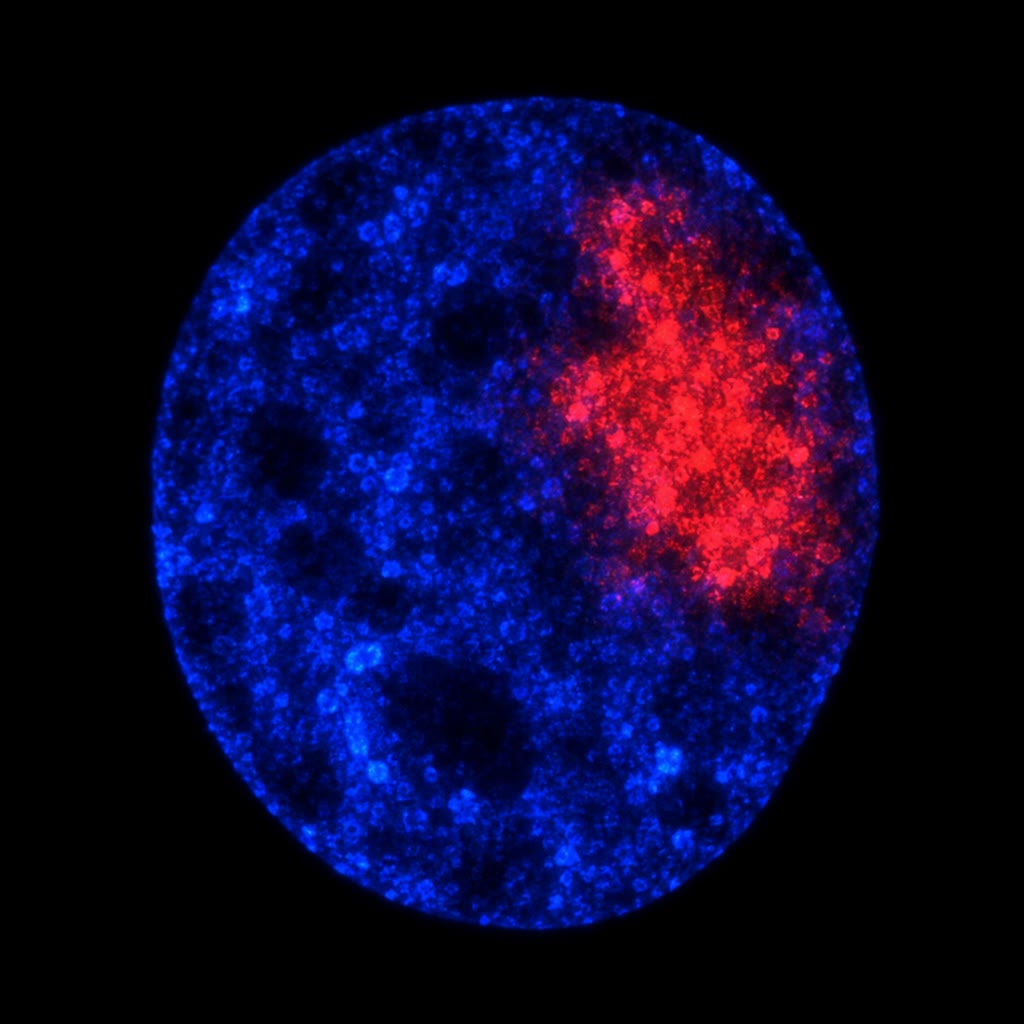
\includegraphics[width=0.36\linewidth]{images/book5/ai/b5-02-lncrna-nucleus.jpg}

{\small काम पर कोई \omterm{def:b3:rna-regulation:ncrna}{दीर्घ अकूटलेखी RNA}: प्रतिदीप्त संकरण से पकड़ा गया
\emph{\omterm{def:b3:chromatin-epigenetics:x-inactivation}{Xist}} अनुलेख (लाल) किसी मादा केंद्रक में एक X गुणसूत्र का
क्षेत्र ढक लेता है (DNA नीले में)।}
\end{omfigure}

\begin{remark}[अनुलेखनोत्तर नियंत्रण से क्या मिलता है]\label{rem:b3:rna-regulation:why}
अनुलेखनी नियंत्रण केंद्रक के रास्ते चलता है, और नया संदेशवाहक बनने,
निर्यात होने तथा अनुवादित होने में मिनटों से घंटों की देरी लगती है।
स्वयं संदेशवाहक का नियंत्रण वहीं चलता है जहाँ प्रोटीन चाहिए, सेकंडों से
मिनटों में, और स्थानिक हो सकता है: कोई अकेली द्रुमिका किसी एक सूत्रयुग्म
पर एक संदेशवाहक का अनुवादन करती हुई, कोई तंतुकोरक जहाँ रेंगता है वहीं
ऐक्टिन बनाता हुआ। वह एक जीन से अनेक प्रोटीन भी बनाता है, और एक ही संकेत
को --- लोहा, कोई अमीनो अम्ल, कोई \omterm{def:b3:rna-regulation:ncrna}{माइक्रो RNA} --- बिना किसी एक प्रवर्तक
को छुए सैकड़ों संदेशवाहकों का समन्वय करने देता है।
\end{remark}

\section{अभ्यास}

\begin{exercise}[$\star$]\label{exo:b3:rna-regulation:1}
miRNA, \omterm{def:b3:rna-regulation:ncrna}{siRNA} और \omterm{def:b3:rna-regulation:ncrna}{piRNA} में उद्गम, लंबाई, डाइसर-निर्भरता और अपने लक्ष्यों
के साथ वे क्या करते हैं, इनके आधार पर भेद कीजिए।
\end{exercise}

\begin{exercise}[$\star$]\label{exo:b3:rna-regulation:2}
किसी \omterm{def:b3:rna-regulation:ncrna}{माइक्रो RNA} का जीवसंश्लेषण उसके जीन से लेकर किसी दमित संदेशवाहक तक
खोजिए, और हर कटाई पर एंज़ाइम का नाम दीजिए।
\end{exercise}

\begin{exercise}[$\star$]\label{exo:b3:rna-regulation:3}
आरंभिक प्रयोगों में कृमियों में \emph{unc-22} का संवेदी RNA अंतःक्षेपित
करने पर जीन क्यों मौन हुआ, और फ़ायर तथा मेलो ने क्या बदला?
\end{exercise}

\begin{exercise}[$\star$]\label{exo:b3:rna-regulation:4}
जब किसी कोशिका को लोहे की भुखमरी दी जाए तो फ़ेरिटिन और ट्रांसफ़ेरिन
ग्राही के साथ क्या होता है? हर स्थिति में अभिव्यक्ति के किस चरण का
नियंत्रण होता है?
\end{exercise}

\begin{exercise}[$\star\star$]\label{exo:b3:rna-regulation:5}
किसी संदेशवाहक का अर्ध-आयु काल \qty{2}{h} है और वह $5$
अणु प्रति मिनट की दर से बनता है। उसका स्थायी-अवस्था स्तर निकालिए, फिर
वह स्तर और अर्ध-काल जब कोई \omterm{def:b3:rna-regulation:ncrna}{माइक्रो RNA} उसकी क्षय-दर दोगुनी कर दे।
\end{exercise}

\begin{exercise}[$\star\star$]\label{exo:b3:rna-regulation:6}
सात न्यूक्लियोटाइड का कोई बीज किसी यादृच्छिक अनुक्रम से प्रायिकता
$4^{-7}$ से मेल खाता है। औसतन \qty{1000}{nt} के 3$'$ अननुवादित
क्षेत्रों वाले \num{20000} संदेशवाहकों के समुच्चय में एक \omterm{def:b3:rna-regulation:ncrna}{माइक्रो RNA}
बीज संयोग से कितने स्थलों से मेल खाएगा? तब किसी वास्तविक लक्ष्य की
पहचान क्या है?
\end{exercise}

\begin{exercise}[$\star\star$]\label{exo:b3:rna-regulation:7}
किसी मक्खी के लिंग का पूर्वानुमान कीजिए: (क) \emph{tra} का
प्रकार्य-ह्रास उत्परिवर्तन और दो X गुणसूत्र; (ख) किसी अनवरत पारजीन से
TRA अभिव्यक्त करती, एक X के साथ; (ग) \emph{dsx} पूरी तरह अनुपस्थित।
\end{exercise}

\begin{exercise}[$\star\star$]\label{exo:b3:rna-regulation:8}
किसी आद्य-कर्कट जीन के संदेशवाहक का अर्ध-आयु काल किसी \omterm{def:b3:rna-regulation:stability}{AU-समृद्ध अवयव}
के कारण सामान्यतः \qty{15}{min} है। कोई गुणसूत्री स्थानांतरण उस अवयव को
हटा देता है और अर्ध-आयु काल \qty{3}{h} हो जाता है। यदि अनुवादन और
प्रोटीन-अपघटन अपरिवर्तित हों तो प्रोटीन का स्तर किस गुणक से बढ़ेगा?
प्रोटीन सामान्य होते हुए भी यह कर्कटजनक क्यों है?
\end{exercise}

\begin{exercise}[$\star\star$]\label{exo:b3:rna-regulation:9}
\emph{Drosophila} की किसी प्रयोगशाला प्रजाति में P अवयव नहीं हैं; किसी
वन्य प्रजाति में हैं। (क) प्रयोगशाला मादाएँ $\times$ वन्य नर,
(ख) वन्य मादाएँ $\times$ प्रयोगशाला नर की संतति की उर्वरता का
पूर्वानुमान कीजिए, और विषमता को \omterm{def:b3:rna-regulation:ncrna}{piRNA} से समझाइए।
\end{exercise}

\begin{exercise}[$\star\star\star$]\label{exo:b3:rna-regulation:10}
\cref{thm:b3:rna-regulation:mirna-kinetics} का उपयोग करते हुए तर्क
दीजिए कि समान माध्य संदेशवाहक स्तर पर, जब संदेशवाहक \omterm{def:b3:rna-regulation:ncrna}{माइक्रो RNA} के
नियंत्रण में हो, तब उससे बना प्रोटीन सापेक्ष रूप में कम उतार-चढ़ाव
करता है। (प्रोटीन संदेशवाहक का अपने ही जीवन-काल पर औसत लेता है, और
संदेशवाहक स्वयं को तेज़ी से नया करता है।) कोई कोशिका वही माध्य पाने के
लिए किसी \omterm{def:b3:rna-regulation:ncrna}{माइक्रो RNA} और ऊँची अनुलेखन-दर का मूल्य क्यों चुकाए?
\end{exercise}

\begin{exercise}[$\star\star\star$]\label{exo:b3:rna-regulation:11}
कृमियों में कोई RNA-निर्भर RNA पॉलीमरेज़ लक्ष्य संदेशवाहक से द्वितीयक
\omterm{def:b3:rna-regulation:ncrna}{siRNA} बनाती है; स्तनधारियों में ऐसी कोई नहीं। हर एक के लिए पूर्वानुमान
कीजिए कि द्विलड़ी RNA के एक ही अंतःक्षेपण से हुआ मौनीकरण अनेक
कोशिका-विभाजनों तक चलता है या नहीं और वह दूसरे ऊतकों में फैलता है या
नहीं, और \omterm{def:b3:rna-regulation:ncrna}{siRNA} औषधों के लिए इसका चिकित्सकीय परिणाम समझाइए।
\end{exercise}

\begin{exercise}[$\star\star\star$]\label{exo:b3:rna-regulation:12}
हृदय में अभिव्यक्त होते किसी नए-टिप्पणीकृत lncRNA के लिए ऐसे प्रयोग
अभिकल्पित कीजिए जो (क) किसी प्रकार्यात्मक RNA, (ख) ऐसे प्रकार्यात्मक
अनुलेखन जिसका RNA अप्रासंगिक है, और (ग) कोलाहल में भेद कर सकें, और
बताइए कि हर एक किस परिणाम का पूर्वानुमान करता है।
\end{exercise}

\section{समस्या: किसी कृमि की घड़ी}

\begin{problem}[{सप्तांत समस्या --- कृमि का \emph{lin-4}/\emph{lin-14}
स्विच संदेशवाहक की गतिकी से समयबद्ध, कोई अंतःक्षेपित RNA किसी भ्रूण के
विभाजनों से तनु होता और प्रवर्धन से बचाया जाता, लौह प्रकार्यगुच्छ का
परिमाणन, और विच्छेदन की एक गणना, जिसका अंत दमन-गुणक, स्विच के अर्ध-काल
और इस पर होता है कि बिना प्रवर्धन कोई संकेत कितने विभाजन जीता है}]
\label{pb:b3:rna-regulation:1}
आँकड़े: \emph{lin-14} संदेशवाहक $k = 3$ अणु प्रति मिनट प्रति कोशिका की
दर से बनता है और उसका अर्ध-आयु काल \qty{40}{min} है। LIN-14 प्रोटीन
$\beta = 2$ प्रति संदेशवाहक प्रति मिनट की दर से बनता है और उसका
अर्ध-आयु काल \qty{3}{h} है। दूसरी डिंभ अवस्था के आरंभ से \emph{lin-4}
RNA जमा होता है और संदेशवाहक पर क्षय-पद $\gamma' R = 3\gamma$ जोड़ता है
और, आरंभन रोककर, $\beta$ को आधा कर देता है। कोई कृमि-भ्रूण एक कोशिका से
बढ़कर अंडे से निकलते समय लगभग \num{550} कोशिकाओं का हो जाता है; किसी
वयस्क में \num{959} कायिक कोशिकाएँ होती हैं।

\medskip
\noindent\textbf{भाग I --- संदेशवाहक।}
\begin{enumerate}
  \item $\gamma$ और \emph{lin-4} के प्रकट होने से पहले का
        स्थायी-अवस्था \emph{lin-14} संदेशवाहक स्तर निकालिए।
  \item प्रोटीन की अपघटन-दर और स्थायी-अवस्था LIN-14 प्रोटीन स्तर
        निकालिए।
  \item \emph{lin-4} के उपस्थित हो जाने पर नया संदेशवाहक स्तर और
        संदेशवाहक का नया काल-नियतांक निकालिए।
  \item नई प्रोटीन स्थायी अवस्था, और प्रोटीन पर कुल दमन-गुणक
        निकालिए।
  \item \emph{lin-4} के प्रकट होने के कितनी देर बाद संदेशवाहक अपने नए
        स्तर तक आधा रास्ता तय कर लेता है? और प्रोटीन --- स्विच की गति
        कौन-सा चरण सीमित करता है?
  \item मूल प्रयोगों में प्रोटीन लुप्त मिला जबकि mRNA अब भी पकड़ में आ
        रहा था। क्या यह आपकी संख्याओं से मेल खाता है? संदेशवाहक का
        कितना अंश बचा रहता है?
\end{enumerate}

\medskip
\noindent\textbf{भाग II --- तनुकरण और प्रवर्धन।}
\begin{enumerate}[resume]
  \item किसी कृमि के जननांग में द्विलड़ी RNA के $10^{6}$ अणु
        अंतःक्षेपित किए जाते हैं, जो \num{250} अंडों में बराबर बँट
        जाते हैं। प्रति अंडा कितने अणु?
  \item यदि अणु हर विभाजन पर बस बाँट दिए जाएँ, तो अंडे से निकलते
        \num{550}-कोशिका वाले कृमि की हर कोशिका में कितने होंगे? और
        कितने विभाजनों के बाद औसत प्रति कोशिका एक से नीचे गिर जाएगा?
  \item फ़ायर और मेलो ने प्रति कोशिका कुछ ही अणुओं पर पूरे प्राणी में
        और उसकी संतति में मौनीकरण देखा। बताइए कि कोई RNA-निर्भर RNA
        पॉलीमरेज़ इस विवरण में क्या जोड़ती है, और फिर भी प्रभाव कुछ
        पीढ़ियों के बाद क्यों मिट जाता है।
  \item ऐसी कोई पॉलीमरेज़ न रखने वाली किसी स्तनधारी कोशिका में \omterm{def:b3:rna-regulation:ncrna}{siRNA}
        अभिवहन \num{5000} युग्मक ऐसी कोशिका में डालता है जो रोज़
        विभाजित होती है; \omterm{def:b3:rna-regulation:rnai}{RISC} स्थिर है पर विभाजन से तनु होता है।
        कितने दिनों बाद संख्या \num{100} से नीचे गिरेगी, जो प्रभावी
        मौनीकरण के लिए मोटे तौर पर आवश्यक संख्या है?
  \item यकृत के किसी संदेशवाहक के विरुद्ध कोई चिकित्सकीय \omterm{def:b3:rna-regulation:ncrna}{siRNA} एक बार
        दिया जाता है और छह महीने काम करता है। यकृत-कोशिकाएँ कम ही
        विभाजित होती हैं। समझाइए कि प्रश्न 10 की क्रियाविधि उसे क्यों
        सीमित नहीं करती, और कौन-सी बात करती है।
  \item सात न्यूक्लियोटाइड का कोई बीज हर $4^{7}$ न्यूक्लियोटाइड पर एक
        बार यादृच्छिक रूप से मेल खाता है। कृमि के अनुलेखितांश में
        लगभग \qty{20}{Mb} 3$'$ अननुवादित अनुक्रम है। \emph{lin-4} के
        कितने संयोगी बीज-मेल हैं, और आनुवंशिकीविदों को कैसे पता चला कि
        कौन-सा लक्ष्य मायने रखता है?
\end{enumerate}

\medskip
\noindent\textbf{भाग III --- लौह प्रकार्यगुच्छ।}
\begin{enumerate}[resume]
  \item लौह-समृद्ध कोशिकाओं में ट्रांसफ़ेरिन ग्राही के संदेशवाहक का
        अर्ध-आयु काल \qty{10}{min} है; IRP बँधा हो तो \qty{50}{min}।
        अनुलेखन अपरिवर्तित रहने पर, लोहा दुर्लभ होने पर संदेशवाहक किस
        गुणक से बढ़ता है?
  \item फ़ेरिटिन संदेशवाहक का स्तर अपरिवर्तित रहता है पर IRP के बँधने
        पर उसका अनुवादन $1$ से घटकर $0.05$ प्रोटीन प्रति संदेशवाहक
        प्रति मिनट रह जाता है। फ़ेरिटिन संश्लेषण किस गुणक से गिरता है?
  \item दोनों को मिलाइए: लौह-समृद्ध और लौह-दरिद्र अवस्थाओं के बीच
        आयात-क्षमता और भंडारण-क्षमता का अनुपात किस गुणक से बदलता है?
  \item IRP1 प्रोटीन या तो RNA-बंधक प्रोटीन है या ऐकोनिटेज़, यह इस पर
        निर्भर करता है कि वह कोई लौह--गंधक गुच्छ धारण करता है या नहीं।
        समझाइए कि इससे वह स्वयं लोहे का संवेदक बनता है, किसी हॉर्मोन
        का नहीं।
  \item किसी रोगी में फ़ेरिटिन IRE का ऐसा उत्परिवर्तन है जो IRP का
        बंधन समाप्त कर देता है। फ़ेरिटिन स्तर, सीरम लोहे और यह
        पूर्वानुमान कीजिए कि नेत्र-लेंस क्यों प्रभावित होता है।
  \item एक वाक्य में समझाइए कि वही हेयरपिन एक स्थान पर सक्रियण और
        दूसरे पर दमन कैसे कर सकती है।
  \item IRP2 में कोई लौह--गंधक गुच्छ नहीं है; लोहा अधिक हो तो उसे कोई
        यूबिक्विटिन लाइगेज़ नष्ट कर देती है जिसके अपने स्थायित्व के
        लिए लोहा और ऑक्सीजन चाहिए। कोई कोशिका इतनी भिन्न रसायन वाले
        दो संवेदक क्यों रखे?
\end{enumerate}

\medskip
\noindent\textbf{भाग IV --- समरूपांतर गिनना।}
\begin{enumerate}[resume]
  \item \emph{Dscam} में परस्पर अपवर्जी 12, 48, 33 और 2 विकल्पों वाले
        बहिर्वेशन-खंड हैं। कितने समरूपांतर? यदि हर तंत्रिका-कोशिका
        यादृच्छिक रूप से लगभग $50$ अभिव्यक्त करे, तो दो दी हुई
        तंत्रिका-कोशिकाओं में कम-से-कम एक साझा होने की प्रायिकता क्या
        है? ($1 - (1 -
        50/N)^{50}$ का उपयोग कीजिए।)
  \item किसी तंत्रिका-कोशिका को ऐसे समरूपांतर रखने से क्या लाभ है जो
        उसके पड़ोसियों के पास लगभग निश्चित रूप से नहीं हैं?
  \item $n$ पेटी-बहिर्वेशनों वाला कोई जीन, जिनमें से हर एक स्वतंत्र
        रूप से समाविष्ट या छोड़ा जाता है, कितने संदेशवाहक देता है?
        $n = 10$ के लिए कितने? किसी दिए हुए कोशिका-प्रकार में
        वास्तविक संख्या प्रायः कहीं कम क्यों होती है?
  \item मक्खी में, दो X गुणसूत्रों पर अकारक \emph{Sxl} युग्मविकल्पी
        वाली कोई मादा केवल नर के रूप में विकसित होने के बजाय मर क्यों
        जाती है? (सोचिए कि X-गणना तंत्र और क्या नियंत्रित करता है:
        X-सहलग्न जीनों का \omterm{def:b3:chromatin-epigenetics:x-inactivation}{मात्रा प्रतिपूरण}।)
  \item SXL अपने ही अनुलेख के उत्पादक विच्छेदन को बढ़ावा देता है।
        समझाइए कि इससे लिंग-निर्णय ऐसी स्मृति कैसे बन जाता है जो
        केवल प्रारंभिक भ्रूण में उपस्थित X-गणना संकेत के जाने के बाद
        भी बनी रहती है, और इसे \cref{ch:b3:chromatin-epigenetics} के
        स्वयं-पोषी स्विचों से जोड़िए।
  \item घड़ी का सारांश दीजिए: LIN-14 प्रोटीन पर दमन-गुणक (प्रश्न~4),
        संदेशवाहक स्विच का अर्ध-काल (प्रश्न~5) और वह संख्या कि बिना
        प्रवर्धन कोई संकेत प्रति कोशिका एक अणु से नीचे गिरने से पहले
        कितने विभाजन जीता है (प्रश्न~8)।
\end{enumerate}
\end{problem}
